
\begin{figure}
  \ContinuedFloat*
  \begin{tabular}[t]{l c}
    \begin{minipage}{0.4\textwidth}
      \begin{Verbatim}[mathescape,commandchars=\\\{\}]
\textbf{dense} 2 2
      \end{Verbatim}
    \end{minipage} & \begin{minipage}{0.4\textwidth}
      \includegraphics[width=\textwidth]{chapters/volr/example2.pdf}
    \end{minipage}

  \end{tabular}
  \caption{A network with a stimulus containing two channels.
    The stimulus is fully connected to a population with an excitatory
    weight of 1. Each circular node represents a single neuron.}
  \label{fig:volr-example1}
\end{figure}

\begin{figure}
  \ContinuedFloat
  \begin{tabular}[t]{l c}
    \begin{minipage}{0.4\textwidth}
      \begin{Verbatim}[mathescape,commandchars=\\\{\}]
\textbf{let} s$_1$ = \textbf{dense} 1 1 \textbf{in}
\textbf{let} s$_2$ = $\neg$ \textbf{dense} 1 1 \textbf{in}
(s$_1$ $\ominus$ s$_2$) $\obar$ \textbf{dense} 2 1
      \end{Verbatim}
    \end{minipage} & \begin{minipage}{0.6\textwidth}
      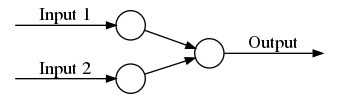
\includegraphics[width=\textwidth]{chapters/volr/example1.pdf}
    \end{minipage}
  \end{tabular}
  \caption{An illustration of a simple binary network, whose two 
	   parallel layers share the middle population of size 2.}
\end{figure}

\begin{figure}
  \ContinuedFloat
  \begin{tabular}[t]{l c}
    \begin{minipage}[b]{0.4\textwidth}
      \begin{Verbatim}[mathescape,commandchars=\\\{\}]
      \textbf{dense} 100 50
        $\obar$ \textbf{dense} 50 10
      \end{Verbatim}
    \end{minipage} & \begin{minipage}{0.5\textwidth}
      \includegraphics[width=\textwidth]{chapters/volr/example3.pdf}
    \end{minipage}
  \end{tabular}
  \caption{A larger network that can process the MNIST dataset
    as 10x10 pixel images. 
    The nodes are populations of neurons,
    where the input corresponds to the pixel size ($10\cdot10=100$) 
    and the output to the possible classes (0 - 9).
    Input and output are implicit.}
\end{figure}

\begin{figure}
  \begin{tabular}[t]{l c}
    \begin{minipage}{0.45\textwidth}
      \begin{Verbatim}[mathescape,commandchars=\\\{\}]
\textbf{let} s = \textbf{dense} 2 2 \textbf{in}
\textbf{let} l$_1$ = \textbf{dense} 2 4 \textbf{in}
\textbf{let} l$_2$ = \textbf{dense} 2 4 \textbf{in}
\textbf{let} o = \textbf{dense} 8 1 \textbf{in} 
  s $\obar$ (l$_1$ $\ominus$ l$_2$) $\obar$ o
      \end{Verbatim}
    \end{minipage} & \begin{minipage}{0.5\textwidth}
       \includegraphics[width=\textwidth]{chapters/volr/example4.pdf}
    \end{minipage}
  \end{tabular}
   \caption{An example where a two-dimensional input is split into
     two nodes and later merged into a node of a single neuron.}
  \label{fig:volr-examples}
\end{figure}
